
This chapter is based on
Ref.\cite{lich-book} by Lichtenberg.

\beq
[\vec{H},\;\cdot\;]E_{\vec{\alp}}
=
[\vec{H}, E_{\vec{\alp}}]= \vec{\alp} E_{\vec{\alp}}
\eeq

\beq
\vec{H}\ket{J, \vec{M}}= \vec{M}\ket{J, \vec{M}}
\eeq


\begin{figure}[h!]
\centering
\includegraphics[width=2.5in]
{weight-diagrams/weight-roots-relation.png}
\caption{Relationship between 2 weights $\vec{M}$ and $\vec{M}'$.}
\label{fig-weight-roots-relation}
\end{figure}



\begin{claim}
For any weight $\vec{M}$ and
root $\vec{\alp}$,
if $k$ is an integer and

\beq k = -\;\frac{2\vec{M}\cdot \vec{\alp}}{\vec{\alp}\cdot\vec{\alp}}
\eeq
then

\beq
\vec{M}'=\vec{M} + k\vec{\alp}
\eeq
is a weight
with the same eigenvalue multiplicity as $\vec{M}$.
\end{claim}
\proof
\qed


\section{WD for $SU(2)$}

\beq
m=-J, -J+1, \ldots, J-1, J
\eeq

\section{WD for $SU(3)$}